\section{Aplicação FTP}

\subsection{Arquitetura da aplicação}

A primeira parte do projeto desenvolvido insidia em criar uma aplicação capaz de executar transferências através de um URL utilizando o protocolo FTP (File Transfer Protocol). No desenvolvimento da aplicação foram tidas em conta as normas \href{https://www.rfc-editor.org/info/rfc959}{RFC959} \href{https://www.rfc-editor.org/info/rfc1738}{RFC1738}, respeitantes à comunicação com o servidor e interpretação do URL respetivamente.

\subsubsection{Interpretação do URL}
A primeira parte da aplicação está responsável por interpretar os argumentos contidos no URL, bem como verificar a sua validade. A função \textbf{create\_url\_data-url\_path\_parser.c}:

\begin{enumerate}
    \item Verifica se o URL corresponde a um protocolo FTP utilizando a função \textbf{is\_ftp}
    \item Interpreta o utilizador e a password presentes (ou não) no URL, que estarão localizadas logo a seguir ao protocolo e separados por ':' e com '@' a marcar o seu fim
    \item Deteta a eventual presença de uma porta com recurso à função \textbf{has\_port} e, em caso positivo, guarda o seu valor
    \item Analiza o caminho e servidor presentes, separa-os, guarda o caminho e o endereço IP com recurso à função \textbf{gethostbyname - netdb.h}
\end{enumerate}

Todos os dados interpretados do URL são guardados numa struct do tipo \textbf{URLPathData}.

\subsubsection{Execução da transferência}
Depois de interpretados os dados do URL necessários para a execução da transferência é necessário comunicar o servidor e efetuar o download do ficheiro pretendido. A função \textbf{ftp\_download - ftp.c}:

\begin{enumerate}
    \item \textbf{ftp\_control\_connect:} Estabelece uma ligação ao servidor (socket) no modo de controlo à porta 21, com recurso à função \textbf{connect - sys/socket.h}
    \item \textbf{ftp\_login:} Efetua autenticação no servidor com as credenciais obtidas pelo URL (comandos USER e PASS e respetivos argumentos são enviados pelo socket)
    \item \textbf{ftp\_retrieve\_passive\_mode:} Envia um pedido de conexão em modo passivo (comando PASV) \textbf{*}
    \item \textbf{ftp\_data\_connect:} Estabelece uma ligação de dados à porta recebida pelo servidor como resposta ao pedido anterior 
    \item \textbf{ftp\_change\_dir\_to\_res:} Na conexão de controlo, muda de diretório para o diretório correto e envia o comando RETR para iniciar o download
    \item \textbf{f\_retrieve\_fd:} Cria um cicheiro local com o mesmo nome do ficheiro remoto
    \item \textbf{ftp\_dump\_data:} Realiza a transferência do ficheiro
    \item \textbf{ftp\_close:} Fecha as conexões com o servidor
\end{enumerate}

Cada pedido ao servidor retorna uma mensagem, da qual retiramos o código através da função \textbf{ftp\_read\_resp\_code}. Este código é interpretado de modo a entender se o procedimento está a seguir o seu curso esperado ou se, a algum momento, houve um erro ou rejeição por parte do servidor.

\textbf{*} em modo passivo, o comando enviado ao servidor é \textbf{PASV} em vez de \textbf{PORT}, sendo o servidor a retornar a porta por onde a ligação de dados deve ser estabelecida e a transferência efetuada

\subsection{Exemplo de Download e Resultados}

A aplicação foi testada com ficheiros de diferentes tamanhos, tipos e de diferentes fontes, sendo experimentado ambos o modo anónimo (sem credenciais) e com autenticação no servidor. Abaixo temos alguns exemplos de execução documentados.

\begin{figure}[!h]
\centering
  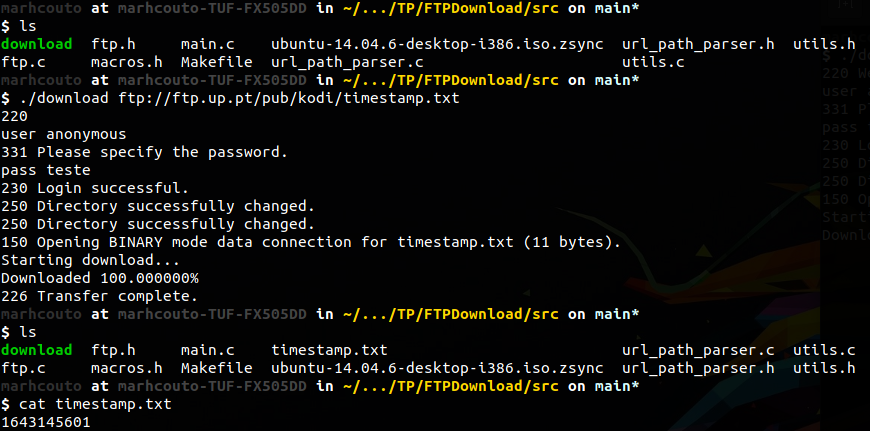
\includegraphics[width=.6\linewidth]{img/Download1.png}
  \caption{Transferência de ficheiro timestamp - 11B}
\end{figure}

\begin{figure}[!h]
\centering
  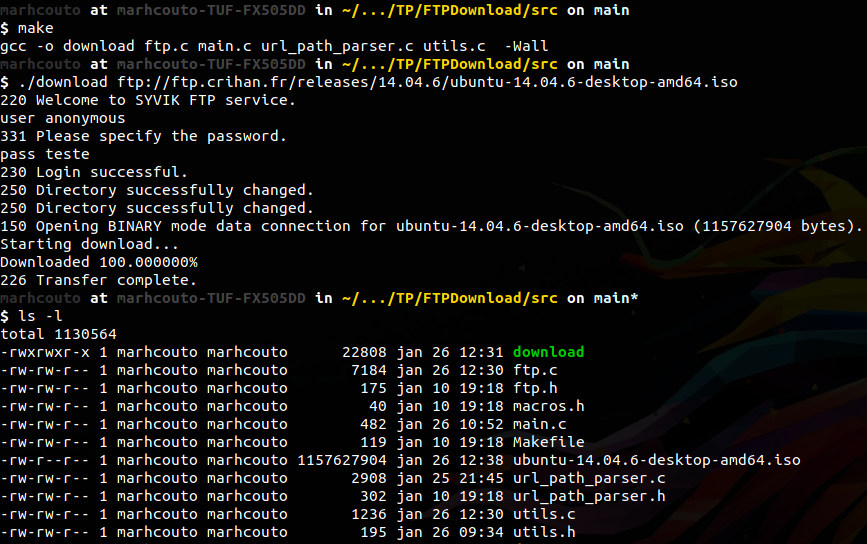
\includegraphics[width=.6\linewidth]{img/Download2.png}
  \caption{Ubuntu iso - 1104 MB}
\end{figure}
